
\documentclass[override]{beamer} %\documentclass[handout]{beamer}
\usetheme{Boadilla} \usecolortheme{crane}
\setbeamertemplate{theorems}[numbered]
\setbeamertemplate{caption}[numbered]
\usepackage[round]{natbib}
\renewcommand{\newblock}{}
%\input{Tex_Commands}
\defbeamertemplate*{footline}{my theme}
{
  \leavevmode%
  \hbox{%
  \begin{beamercolorbox}[wd=.333333\paperwidth,ht=2.25ex,dp=1ex,center]{author in head/foot}%
    \usebeamerfont{author in head/foot}\insertshortauthor~~(\insertshortinstitute)
  \end{beamercolorbox}%
  \begin{beamercolorbox}[wd=.333333\paperwidth,ht=2.25ex,dp=1ex,center]{title in head/foot}%
    \usebeamerfont{title in head/foot}\insertshorttitle
  \end{beamercolorbox}%
  \begin{beamercolorbox}[wd=.333333\paperwidth,ht=2.25ex,dp=1ex,right]{date in head/foot}%
    \usebeamerfont{date in head/foot}\insertshortdate{}\hspace*{2em}
    \insertframenumber{}\hspace*{2ex} 
  \end{beamercolorbox}}%
  \vskip0pt%
}
\newcommand{\Span}{\mathrm{span}}
\newcommand{\rank}{\mathrm{rank}}
\newcommand{\evdeq}{\overset{\mathrm{EVD}}=} %{\stackrel{EVD}{=}}
\newcommand{\svdeq}{\overset{\mathrm{SVD}}=} %{\stackrel{EVD}{=}}
\newcommand{\bi}{\begin{itemize} \scriptsize} \newcommand{\ei}{\end{itemize}}
\newcommand{\ben}{\begin{enumerate} \scriptsize} \newcommand{\een}{\end{enumerate}}
\newcommand{\vs}{\vspace{0.1in}}
\newcommand{\vsl}{\vspace{0.05in}}
\newcommand{\vsm}{\vspace{-0.1in}}

\usepackage{amsmath,array,graphicx,float,amssymb,bm,bbm} %,tabu,setspace}
\usepackage{subcaption}
%\usepackage{algorithmic}
%\usepackage{algorithm}
\usepackage{epsfig,epstopdf} %etex,
\usepackage{graphicx} % Allows including images
\usepackage{booktabs} % Allows the use of \toprule, \midrule and \bottomrule in tables
%\usepackage{times}

\usepackage{mathtools, amsthm}
\usepackage{amsmath}
\usepackage{amssymb}
\usepackage{amsbsy}
\usepackage{enumerate}
\usepackage{array}
\usepackage{times}
\usepackage{latexsym}
\usepackage{graphics}
\usepackage{graphicx}
\usepackage{undertilde}
\usepackage{accents}
\usepackage{color}
\usepackage{mathrsfs}
\usepackage{url}
\usepackage{wrapfig}
%% Packages
\usepackage{amsfonts}
\usepackage{amssymb}
\usepackage{amsthm}
\usepackage{booktabs}
\usepackage{color}
\usepackage{enumerate,verbatim}
\usepackage[sf,small,center, compact]{titlesec}
\usepackage{float}
\usepackage{hyperref}
\usepackage{ulem}
\usepackage{array}
\usepackage{url}
\usepackage{threeparttable}
\usepackage{multirow}
\usepackage{wrapfig}
\usepackage{lscape}
\usepackage{rotating}
\usepackage{epstopdf}

\usepackage{ulem}
\usepackage{algorithm2e}
\theoremstyle{remark}


\newcommand{\bs}[1]{{\boldsymbol{#1}^*}}
\newcommand{\bb}[1]{{\boldsymbol {#1}}}

\renewcommand{\bm}{\mathbf}
\newcommand{\x}{\bm{x}}
\newcommand{\e}{\bm{e}}
\newcommand{\y}{\bm{y}}
\newcommand{\w}{\bm{w}}
\newcommand{\X}{\bm{X}}
\newcommand{\U}{{\bm{U}}}
\newcommand{\R}{{\bm{R}}}
\newcommand{\G}{\bm{G}}

\newcommand{\I}{\bm{I}}
\newcommand{\Y}{\bm{Y}}
\newcommand{\s}{\bm{s}}
\newcommand{\uhat}{{\bm{\u}}}
\newcommand{\Zhat}{{\bm{\hat{Z}}}}
\newcommand{\Z}{{\bm{{Z}}}}
\newcommand{\D}{{\bm{D}}}
\newcommand{\Q}{{\bm{Q}}}
\newcommand{\F}{{\bm{F}}}
\newcommand{\iidsim}{\stackrel{\mathrm{iid}}{\thicksim }}
\newcommand{\indepsim}{\stackrel{\mathrm{indep.}}{\thicksim }}
\newcommand{\SE}{\scriptsize{\mathrm{SubsDist}}}  %{\sin\theta_{mx}}
\newcommand{\dist}{\mathrm{dist}}
\newcommand{\tta}{\ta^{\text{trunc}}}
\newcommand{\A}{\bm{A}}
\newcommand{\full}{{\mathrm{full}}}
\newcommand{\cb}{\bm{c}}



\setlength{\arraycolsep}{0.01cm}%{0.03cm}

\newcommand{\n}{\mathcal{N}}
\newcommand{\matdist}{\text{mat-dist}}
\newcommand{\outfrac}{\text{\scriptsize{max-outlier-frac}}}
\newcommand{\outfracrow}{\text{\scriptsize{max-outlier-frac-row}}}
\newcommand{\outfraccol}{\text{\scriptsize{max-outlier-frac-col}}}
\newcommand{\missfracrow}{\text{\scriptsize{max-miss-frac-row}}}
\newcommand{\missfraccol}{\text{\scriptsize{max-miss-frac-col}}}


\newcommand{\xmint}{\x_{\min}}%{\text{\scriptsize{min-outlier-mag}}}%{\x_{\min}}%
\newcommand{\rmat}{r_{\scriptscriptstyle{L}}}
\newcommand{\tmax}{d}
\newcommand{\that}{\hat{t}}
\newcommand{\train}{\text{train}}

%\newcommand{\bea}{\begin{align*}}  \newcommand{\eea}{\end{align*}}
\newcommand{\bea}{\begin{eqnarray} }
\newcommand{\eea}{\end{eqnarray} }

\newcommand{\nn}{\nonumber}
\newcommand{\hd}{\frametitle}
\renewcommand{\S}{\mathcal{S}}
\newcommand{\deltatfrob}{\delta_{t}}
\newcommand{\deltainitfrob}{\delta_{0}}
\renewcommand{\S}{\mathcal{S}}
\newcommand{\g}{\bm{g}}
\newcommand{\Bhat}{\hat\B}
%\newcommand{\M}{\bm{M}}
\newcommand{\SEF}{\SE}
%\newcommand{\G}{\bm{G}}
\newcommand{\eps}{\epsilon}
%\input{tikz_defs}
\usepackage{tikz}
\usepackage{pgfplots}
\usepgfplotslibrary{groupplots}

%\usepackage{subfig}

\usepackage{tikz}
\usepackage{pgfplots}
%\usepackage{pgfplotstable}
\usepgfplotslibrary{groupplots}
\usepackage{multirow,multicol}

%\renewcommand{\x}{\bm{x}} \renewcommand{\X}{\bm{X}}

\newcommand{\xhat}{\hat\x}
\newcommand{\Xhat}{\hat\X}


\def\red{\textcolor{red}}

\begin{document}

\title[Matrix Completion]{Matrix Completion}

\subtitle{A brief overview of Section 3.8 of \cite{Chen:2021}}
\author[Zhiling Gu]{Zhiling Gu} % Your name
\institute[Iowa State U.]{Iowa State University}
\date{\today}


\begin{frame}[plain]
\titlepage

%\scriptsize
%\vs
%\tiny
%based on first 4 chapters of the book ``High Dimensional Probability for Data Science'' and the tutorial article on ``Non-asymptotic Random Matrix Theory'' by Roman Vershynin
%\\
%\vs
\end{frame}
%\input{intro_slides}

%\begin{frame}
%\scriptsize
%\frametitle{\small Tutorial Outline}
%\tableofcontents
%\vs
%\end{frame}





\begin{frame} [allowframebreaks,squeeze]
\frametitle{Motivation}
In the practice, it is extremely common to encounter missing data due to collection difficulty, erroneous data, and etc.
And most of the data can be represented in the matrix. For example, if we consider each row of a matrix is the features/ measurements of a single subject, a matrix would represent the features of all the subjects/ population of interest.
To tackle the missing data problem, one of the tool is matrix completion. 

\begin{figure}
    \centering
    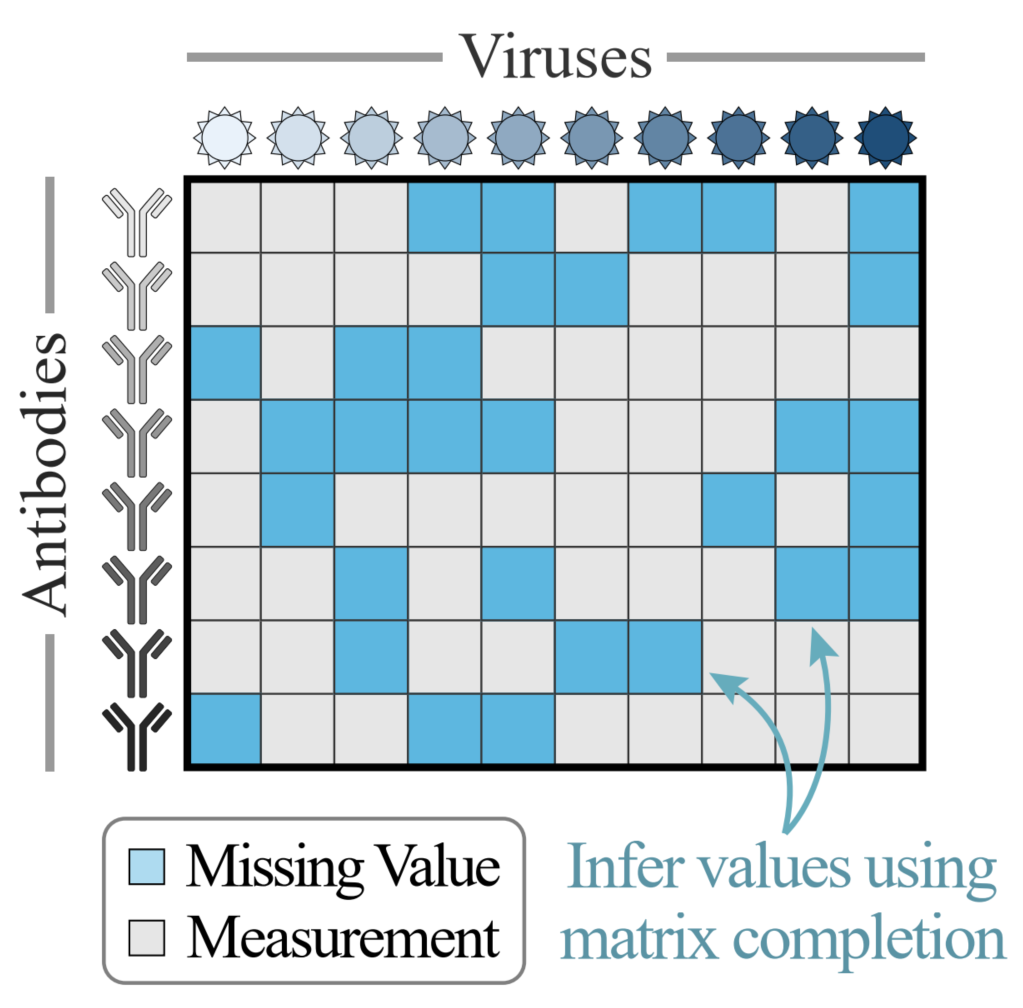
\includegraphics[width = 0.5 \textwidth]{einav-image.png}
    \caption{source: \url{https://www.fredhutch.org/en/news/spotlight/2022/08/bs-einav-cellsys.html}}
\end{figure}
\end{frame}

\begin{frame}[allowframebreaks,squeeze]
\frametitle{Preparation}
\textbf{Norms}
\bi
\item For any vector $\boldsymbol{v}$, we denote by $\|\boldsymbol{v}\|_2,\|\boldsymbol{v}\|_1$ and $\|\boldsymbol{v}\|_{\infty}$ its $\ell_2$ norm, $\ell_1$ norm and $\ell_{\infty}$ norm, respectively. 

\item For any matrix $\boldsymbol{A}=\left[A_{i, j}\right]_{1 \leq i \leq m, 1 \leq j \leq n}$, we let $\red{\|\boldsymbol{A}\|},\|\boldsymbol{A}\|_*$, $\|\boldsymbol{A}\|_{\mathrm{F}}$ and $\|\boldsymbol{A}\|_{\infty}$ represent respectively its \red{spectral norm (i.e., the largest singular value of $\boldsymbol{A}$ )}, its nuclear norm (i.e., the sum of singular values of $\boldsymbol{A}$ ), its Frobenius norm (i.e., $\|\boldsymbol{A}\|_{\mathrm{F}}:=\sqrt{\sum_{i, j} A_{i, j}^2}$ ), and its entrywise $\ell_{\infty}$ norm (i.e., $\left.\|\boldsymbol{A}\|_{\infty}:=\max _{i, j}\left|A_{i, j}\right|\right)$. We also refer to $\|\boldsymbol{A}\|_{2, \infty}$ as the $\ell_{2, \infty}$ norm of $\boldsymbol{A}$, defined as $\|\boldsymbol{A}\|_{2, \infty}:=\max _i\left\|\boldsymbol{A}_{i, \cdot}\right\|_2$. Similarly, we define the $\ell_{\infty, 2}$ norm of $\boldsymbol{A}$ as $\|\boldsymbol{A}\|_{\infty, 2}:=\left\|\boldsymbol{A}^{\top}\right\|_{2, \infty}$.
\item Singular values of $\bb M$  are square roots of the eigenvalues of $\bb M^H \bb M$.
\item The largest singular value $\sigma_1(\bb M)$= operator norm $\|\bb M\|_{op} := \max_{\|x\|_2= 1} \|\bb Mx\|_2$.
\item In addition, for any matrices $\boldsymbol{A}=\left[A_{i, j}\right]_{1 \leq i \leq m, 1 \leq j \leq n}$ and $\boldsymbol{B}=\left[B_{i, j}\right]_{1 \leq i \leq m, 1 \leq j \leq n}$, the inner product of $\boldsymbol{A}$ and $\boldsymbol{B}$ is defined as and denoted by $\langle\boldsymbol{A}, \boldsymbol{B}\rangle=\sum_{1 \leq i \leq m, 1 \leq j \leq n} A_{i, j} B_{i, j}=\operatorname{Tr}\left(\boldsymbol{A}^{\top} \boldsymbol{B}\right)$.
\ei

Consider $\bb M = \bs M + \bb E$ and $\bs M$ be two matrices of $\mathbb R^{n_1\times n_2}$, $n_1\leq n_2$.
Let $\bs M = \bs U \bs \Sigma \bs V$, $\bb M = \bb U \bb \Sigma \bb V$ as follows

$$
\begin{gathered}
\bs M=\sum_{i=1}^{n_1} \sigma_i^{\star} u_i^{\star} \boldsymbol{v}_i^{\star \top}=\left[\begin{array}{ll}
\bs U & \bs U_{\perp}
\end{array}\right]\left[\begin{array}{ccc}
\bs \Sigma & 0 & 0 \\
0 & \bs \Sigma_{\perp}& 0
\end{array}\right]\left[\begin{array}{c}
\boldsymbol{V}^{\star \top} \\
\boldsymbol{V}_{\perp}^{\star \top}
\end{array}\right] ; \\
\bb M=\sum_{i=1}^{n_1} \sigma_i \boldsymbol{u}_i \boldsymbol{v}_i^{\top}=\left[\begin{array}{ll} \red{\bb U} & \bb U_{\perp}
\end{array}\right]\left[\begin{array}{ccc}
\red{\bb \Sigma} & 0 & 0 \\
0 & \boldsymbol{\Sigma}_{\perp} & 0
\end{array}\right]\left[\begin{array}{c}
\red{\boldsymbol{V}^{\top}} \\
\boldsymbol{V}_{\perp}^{\top}
\end{array}\right] .
\end{gathered}
$$
Here, $\sigma_1 \geq \cdots \geq \sigma_{n_1}$ (resp. $\sigma_1^{\star} \geq \cdots \geq \sigma_{n_1}^{\star}$ ) stand for the singular values of $M$ (resp. $\left.M^{\star}\right)$ arranged in descending order, $\boldsymbol{u}_i$ (resp. $\left.\boldsymbol{u}_i^{\star}\right)$ denotes the left singular vector associated with the singular value $\sigma_i\left(\right.$ resp. $\left.\sigma_i^{\star}\right)$, and $\boldsymbol{v}_i$ (resp. $\left.\boldsymbol{v}_i^{\star}\right)$ represents the right singular vector associated with $\sigma_i\left(\right.$ resp. $\left.\sigma_i^{\star}\right)$. In addition, we denote
$$
\begin{aligned}
\boldsymbol{\Sigma} &:=\operatorname{diag}\left(\left[\sigma_1, \cdots, \sigma_r\right]\right), & \boldsymbol{\Sigma}_{\perp} &:=\operatorname{diag}\left(\left[\sigma_{r+1}, \cdots, \sigma_{n_1}\right]\right), \\
\boldsymbol{U} &:=\left[\boldsymbol{u}_1, \cdots, \boldsymbol{u}_r\right] \in \mathbb{R}^{n_1 \times r}, & \boldsymbol{U}_{\perp} &:=\left[\boldsymbol{u}_{r+1}, \cdots, \boldsymbol{u}_{n_1}\right] \in \mathbb{R}^{n_1 \times\left(n_1-r\right)}, \\
\boldsymbol{V} &:=\left[\boldsymbol{v}_1, \cdots, \boldsymbol{v}_r\right] \in \mathbb{R}^{n_2 \times r}, & \boldsymbol{V}_{\perp} &:=\left[\boldsymbol{v}_{r+1}, \cdots, \boldsymbol{v}_{n_2}\right] \in \mathbb{R}^{n_2 \times\left(n_2-r\right)}
\end{aligned}
$$
The matrices $\boldsymbol{\Sigma}^{\star}, \boldsymbol{\Sigma}_{\perp}^{\star}, \boldsymbol{U}^{\star}, \boldsymbol{U}_{\perp}^{\star}, \boldsymbol{V}^{\star}, \boldsymbol{V}_{\perp}^{\star}$ are defined analogously.

In addition, we define the distance between two matrices as 
\begin{equation}
\begin{aligned}
\operatorname{dist}\left(\boldsymbol{U}, \boldsymbol{U}^{\star}\right) &:=\min _{\boldsymbol{R} \in \mathcal{O}^{r \times r}}\left\|\boldsymbol{U} \boldsymbol{R}-\boldsymbol{U}^{\star}\right\| 
% \operatorname{dist}_{\mathrm{F}}\left(\boldsymbol{U}, \boldsymbol{U}^{\star}\right) &:=\min _{\boldsymbol{R} \in \mathcal{O}^{r \times r}}\left\|\boldsymbol{U} \boldsymbol{R}-\boldsymbol{U}^{\star}\right\|_{\mathrm{F}}
\end{aligned}
\end{equation}
\end{frame}



\begin{frame}[allowframebreaks,squeeze]
\frametitle{Problem formulation and assumption}
Suppose the data matrix $\mathbf M^*$ is of dimension $n_1\times n_2$ with rank $r$.
Assume \[n_1\leq n_2.\]
We start with the single value decomposition of $\bs M$ as follows
\[
\bs M = \bs U \bs \Sigma \bs V^\top,
\]
where $col(\bs U) \in \mathbb R^{n_1\times r}, col(\bs V) \in \mathbb R^{n_2\times r}$, and $\bs \Sigma$ is a diagonal matrix with entries singular values, denoted as $\sigma_1(\bs M), \ldots, \sigma_r(\bs M)$ in descending order.
And we introduce \red{\textit{condition number}} of matrix $\bs M$ to be 
\[
\kappa := \sigma_1(\bs M)/\sigma_r(\bs M),
\]
and we define an index subset $\Omega \subset [n_1]\times [n_2]$ such that $(i,j)\in\Omega \iff \bs M_{ij}$ is observed.

\noindent\textbf{Assumption 1} (Random sampling). 
In this report, we assume each entry of $\bs M$ is observed independently with probability $0<p<1$. 
This corresponds to \textit{missing at random} in statistics terminology.

\noindent\textbf{Example} (Incoherence).
Here we provide an example that satisfies random sampling but causes unfaithful recovery.
Consider $\bs M$ being a zero matrix except for 1 entry. If $p = o(1)$, then with high probability, the single nonzero entry would be missing, and any recovery method would be in vain to recover the rank $1$ property.
$$
\begin{pmatrix}
\red{1}& 0 & 0 & 0 & 0 \\
0 & 0 & 0 & 0 & 0 \\
0 & 0 & 0 & 0 & 0\\
0 & 0 & 0 & 0 & 0\\
0 & 0 & 0 & 0 & 0
\end{pmatrix}
$$

\newpage
\noindent \textbf{$\mu$-incoherent}.
Motivated by the previous example, we define the \red{\textit{incoherence parameter}} $\mu$ of $\bs M$ as follows
\[
\mu:= \max\left\{
\frac{n_1\|\bs U\|_{2,\infty}^2}{r},
 \frac{n_2\|\bs V\|_{2,\infty}^2}{r}
 \right\}.
\]

Recall that 
$\|\bs U\|_{2,\infty} = \max_i\|\bs U_{i,\cdot}\|_2$ is the largest $\ell_2$ norm among rows of $\bs U$.
Also note by SVD, $\bs U$ and $\bs V$ are unitary matrices, and thus $\bs U\bs U^\top = \mathbf I_r$ leading to $\|\bs U\|_F^2 = r$.
\[
\frac{r}{n_1} = \frac{1}{n_1}\|\bs U\|_F^2
\leq 
\|\bs U\|_{2,\infty}^2
\leq\|\bs U\|^2 = 1
\]
\[
\implies
1\leq \mu\leq \max\{n_1, n_2\} /r = n_2/r.
\]
\red{A smaller $\mu$ indicates the energy of singular vectors is spread out across different elements.}
\end{frame}


\begin{frame}[allowframebreaks,squeeze]
\frametitle{Algorithm}

\noindent \textbf{Euclidean projection operator: $\mathcal P_\Omega: \mathbb R^{n_1\times n_2}\to \mathbb R^{n_1\times n_2}$}.
It is now natural to define a projection from original space $\mathbb R^{n_1\times n_2}$ where $\bs M$ lies in a subspace of $\mathbb R^{n_1\times n_2}$ as follows:
$$
[\mathcal P_{\Omega} (\bs M)]_{ij} = 
\begin{cases}
\bs M_{ij}, &\mathrm{ if } (i,j)\in\Omega\\
0, &\mathrm{ else.}
\end{cases}
$$
And our goal is to recover $\bs M$ on the basis of $\mathcal P_\Omega (\bs M)$.

\textbf{Example:}
\begin{align*}
    \text{Observed matrix}
    =
    \begin{pmatrix}
    1 & \red{?} & \red{?} & 2 \\
    2& 1 & 3& 1\\
    4 & 1& 1& \red{?}
    \end{pmatrix}
    \\
     \mathcal P_\Omega(\bs M)
    =
    \begin{pmatrix}
    1 & \red{0} & \red{0} & 2 \\
    2& 1 & 3& 1\\
    4 & 1& 1& \red{0}
    \end{pmatrix}
\end{align*}
\newpage 
\textbf{Algorithm:} 
Under the assumption of random sampling, we consider an approximation $\bs M$, $\bb M$, through \textit{inverse probability weighting} of observed data matrix
\begin{align}
    \bb{M}:= p^{-1} \mathcal P_\Omega (\bs {M}).
\end{align}
Since the observed data is in the random subspace $\mathcal P_\Omega (\bs {M})$, 
$\bb M$ is in fact a random approximation matrix.
This construction leads to
$$\mathbb E_\Omega (\bb M) = \bs M.$$

Then
we compute \red{rank-$r$} SVD of $\bb M = \bb U \bb \Sigma \bb V^\top$,
and 
$\bb U, \bb V$ are employed as the estimates of 
$\bs U, \bs V$, respectively.
\end{frame}

\begin{frame}{Example of inverse probability weighting}
\begin{align*}
     \text{True matrix } 
     \bs M
    =
    \begin{pmatrix}
    1 & \red{2} & \red{2} & 2 \\
    2& 1 & 3& 1\\
    4 & 1& 1& \red{3}
    \end{pmatrix}\\
    \text{Observed matrix}
    =
    \begin{pmatrix}
    1 & \red{?} & \red{?} & 2 \\
    2& 1 & 3& 1\\
    4 & 1& 1& \red{?}
    \end{pmatrix}
    \\
     \mathcal P_\Omega(\bs M)
    =
    \begin{pmatrix}
    1 & \red{0} & \red{0} & 2 \\
    2& 1 & 3& 1\\
    4 & 1& 1& \red{0}
    \end{pmatrix}\\
    \text{Approximation matrix } 
    \bb{M}:= p^{-1} \mathcal P_\Omega (\bs {M}) 
\end{align*}
Assume $p$ and $r$ are known. $\bb U\bb\Sigma \bb V$ is the rank-$r$ SVD of $\mathbf M$.

We ask: how close is $\bb U\bb\Sigma \bb V$ and $\bs M$?
\end{frame}


\begin{frame}
\frametitle{Useful bounds of matrix norms}
\begin{lemma}[Lemma 3.20 of \cite{Chen:2021}]
\label{LEM1}
Assume $\bs M \in \mathbb{R}^{n_1\times n_2}$ is $\mu$-coherent. Then the following relations holds
\begin{align}
    \|\bs M\|_{2,\infty} \leq \sqrt{\mu r/n_1}\|\bs M\|\\
     \|\bs M^\top\|_{2,\infty} \leq \sqrt{\mu r/n_2}\|\bs M\|\\
      \|\bs M\|_{\infty} \leq \mu r\sqrt{1/n_1n_2}\|\bs M\|.
\end{align}
\end{lemma}

\end{frame}



\begin{frame}
\frametitle{Perturbation bound of $\bb M$}
\begin{lemma}[Lemma 3.21 of \cite{Chen:2021}]
\label{LEM2}
Suppose $n_2 p\geq C\mu r\log n_2$ for some constant $C>0$, then with probability at least $1-O(n_2^{-10})$, one has 
\[
\|\bb M -\bs M\| 
\lesssim
\sqrt{\frac{\mu r\log n_2}{n_1 p}} \|\bs M\|.
\]
\end{lemma}
The higher the probability of observation $p$ is, the better the bound is.
\end{frame}



\begin{frame}
\frametitle{Recovery of $\boldsymbol {U}, \boldsymbol {V}$}
\begin{theorem}[Theorem 3.22 of \cite{Chen:2021}]
\label{THM1}
Suppose $n_1 p\geq C \kappa^2 \mu r\log n_2$ for some constant $C>0$, then with probability at least $1-O(n_2^{-10})$, one has
$$
\max \left\{\operatorname{dist}\left(\boldsymbol{U}, \boldsymbol{U}^{\star}\right), \operatorname{dist}\left(\boldsymbol{V}, \boldsymbol{V}^{\star}\right)\right\}  
\lesssim
 \kappa \sqrt{\frac{\mu r \log n_2}{n_1 p}}.
$$
\end{theorem}
Note that when the sample size $pn_1 n_2 \gg \kappa^2 \mu r n_2 \log n_2$, the spectral estimate achieves consistent estimation $\max \left\{\operatorname{dist}\left(\boldsymbol{U}, \boldsymbol{U}^{\star}\right), \operatorname{dist}\left(\boldsymbol{V}, \boldsymbol{V}^{\star}\right)\right\} = o_p(1)$.

\end{frame}



\begin{frame}
\frametitle{Recovery of $\boldsymbol M$}
\begin{theorem}[Theorem 3.23 of \cite{Chen:2021}]
\label{THM2}
Suppose $n_2 p\geq C\mu r\log n_2$ for some constant $C>0$, then with probability at least $1-O(n_2^{-10})$, one has 
\[
\|\bb U\bb \Sigma \bb V^{\top} 
- \bs M\|_F 
\lesssim
\sqrt{\frac{\mu r^2\log n_2}{n_1 p }} \|\bs M\|
\]
\end{theorem}
The theorem above only requires Lemma \ref{LEM2} and characterizes the statistical accuracy of $\bb U\bb \Sigma \bb V^\top$.

\end{frame}



\begin{frame}
\frametitle{Wedin's Theorem}
\begin{theorem}[Wedin  $\sin \Theta$ theorem for singular subspace perturbation, Theorem 3.22 of \cite{Chen:2021}]
If $\|\boldsymbol{E}\|<\sigma_r^{\star}-\sigma_{r+1}^{\star}$, then one has
$$
\begin{aligned}
\max \left\{\operatorname{dist}\left(\boldsymbol{U}, \boldsymbol{U}^{\star}\right), \operatorname{dist}\left(\boldsymbol{V}, \boldsymbol{V}^{\star}\right)\right\} & \leq \frac{\sqrt{2} \max \left\{\left\|\boldsymbol{E}^{\top} \boldsymbol{U}^{\star}\right\|,\left\|\boldsymbol{E} \boldsymbol{V}^{\star}\right\|\right\}}{\sigma_r^{\star}-\sigma_{r+1}^{\star}-\|\boldsymbol{E}\|}.
% \max \left\{\operatorname{dist}_{\mathrm{F}}\left(\boldsymbol{U}, \boldsymbol{U}^{\star}\right), \operatorname{dist}_{\mathrm{F}}\left(\boldsymbol{V}, \boldsymbol{V}^{\star}\right)\right\} & \leq \frac{\sqrt{2} \max \left\{\left\|\boldsymbol{E}^{\top} \boldsymbol{U}^{\star}\right\|_{\mathrm{F}},\left\|\boldsymbol{E} \boldsymbol{V}^{\star}\right\|_{\mathrm{F}}\right\}}{\sigma_r^{\star}-\sigma_{r+1}^{\star}-\|\boldsymbol{E}\|} .
\end{aligned}
$$
\end{theorem}
\end{frame}



\begin{frame}[allowframebreaks,squeeze]
\frametitle{Proof of Theorem 3.22 of \cite{Chen:2021}}
\bi
\item 
Sketch of the proof: 
(i) Prove $\bb E = \bb M - \bs M$ satisfy $\|\bb E\| < \sigma_r(\bs M) - \sigma_{r+1}(\bs M)$, where $\sigma_r(\bs M)$ is the r-th largest singular value of $\bs M$. (ii) Apply Wedin's theorem to $\bb E$ and use lemma \ref{LEM2}.
\item
Step (i): recall $n_1 \geq n_2$, thus the condition of lemma \ref{LEM2} is satisfied. Then 
\begin{align*}
    \|\bb E\| = \|\bb M  - \bs M\| 
    \lesssim \sqrt{\frac{\mu r \log n_2}{n_1 p }} \|\bs M\|.
\end{align*}
In addition, recall that $\sigma_1(\bs M) = \|\bs M\| = \kappa \sigma_r(\bs M)$ by definition of singular value and $\kappa$.
Therefore 
\begin{align*}
    \|\bb E\| 
    \lesssim & \sqrt{\frac{\mu r \log n_2}{n_1 p }} \|\bs M\|
    = \sqrt{\frac{ \kappa^2 \mu r \log n_2}{n_1 p }} \sigma_r(\bs M) \\
    \leq & \frac{1}{C} \sigma_r(\bs M) \text{ for some large enough $C>0$}.
\end{align*}
Choose $C$ such that $1/C < 1-1/\sqrt{2}$, we have 
\begin{align*}
    \|\bb E\| 
    \lesssim 
    (1-\frac{1}{\sqrt{2}}) \sigma_r(\bs M).
\end{align*}
Note we can always choose a large enough $C$ such that the condition of Wedin's theorem $\|\bb E\| < \sigma_r(\bs M) - \sigma_{r+1}(\bs M) $ holds.

\item
Step (ii): Apply Wedin's theorem to $\bb E$, we have 
\begin{align*}
& \max \left\{\operatorname{dist}\left(\boldsymbol{U}, \boldsymbol{U}^{\star}\right), \operatorname{dist}\left(\boldsymbol{V}, \boldsymbol{V}^{\star}\right)\right\} \\
& \leq \frac{\sqrt{2} \max \left\{\left\|\boldsymbol{E}^{\top} \boldsymbol{U}^{\star}\right\|,\left\|\boldsymbol{E} \boldsymbol{V}^{\star}\right\|\right\}}{\sigma_r(\bs M)-\sigma_{r+1}(\bs M)-\|\boldsymbol{E}\|} \text{ by  Wedin's theorem}\\
&  \leq \frac{\sqrt{2} \|\bb E\| \max \left\{\left\|\boldsymbol{U}^{\star}\right\|,\left\|\boldsymbol{V}^{\star}\right\|\right\}}{\sigma_r(\bs M)-\|\boldsymbol{E}\|} \text{ by } \|AB\|\leq \|A\|\|B\|\\
& \leq \frac{\sqrt{2} \|\bb E\|}{\sigma_r^{\star}-(1-\frac{1}{\sqrt{2}})\sigma_r(\bs M)} \text{ by unitary matrix $\bs U, \bs V$}\\
& = 2 \|\bb E\| / \sigma_r(\bs M) 
= 2\kappa \|\bb E\| /\sigma_1(\bs M)\\
& \lesssim \kappa \sqrt{\frac{\mu r\log n_2}{n_1 p}} \text{ by Lemma \ref{LEM2}}.
\end{align*}
\ei
\end{frame}




\begin{frame}
\frametitle{Proof of Theorem 3.23 of \cite{Chen:2021}}
\bi
\item By triangle inequality, we have
\[
\|\bb U\bb \Sigma \bb V^\top - \bs M\|
\leq
\|\bb U\bb \Sigma \bb V^\top - \bb M\| +\|\bb M - \bs M\|.
\]
Note that $\bb U\bb \Sigma \bb V^\top$ is the SVD of $\bb M$ and thus the best rank-$r$ approximation to $\bb M$. 
Therefore $\|\bb U\bb \Sigma \bb V^\top - \bb M\| \leq \|\bb M - \bs M\|$, where $\bs M$ is an unknown rank-$r$ matrix.
\item 
In addition, since both $\bb U\bb \Sigma \bb V^\top $ and $\bs M$ are of rank $r$, the difference between them would have rank at most $2r$. This leads to 
\begin{align*}
\|\bb U\bb \Sigma \bb V^\top - \bs M\|
& \leq
\|\bb U\bb \Sigma \bb V^\top - \bb M\| +\|\bb M - \bs M\|\\
& \leq 2\|\bb M - \bs M\| \\
\|\bb U\bb \Sigma \bb V^\top - \bs M\|_F
& \leq \sqrt{2r} \|\bb U\bb \Sigma \bb V^\top - \bs M\| \text{ by Remark *} \\
& \leq 2\sqrt{2r} \|\bb M - \bs M\|\\
& \lesssim \sqrt{\frac{\mu r^2 \log n_2}{n_1 p }} \|\bs M\| \text{ by Lemma \ref{LEM2}}.
\end{align*}
\item Remark *:$ \|\bb M\|_F\leq \sqrt{r}\|\bb M\| $. This can be proved as follows.
$\|\bb M\|_F = \sqrt{\sum_{i} (\bb e_i^\top \bb M^\top \bb M \bb e_i)} 
= \sqrt{\sum_{i} (\bb e_i^\top \bb U \bb \Sigma^2 \bb V^\top \bb e_i)}
\leq \sqrt{\sum_{i = 1}^r\|\bb e_i^\top \bb U\|_2 \|\bb M\|^2 \|\bb V ^\top \bb e_i\|_2 }
= \sqrt{r}\|\bb M\|
$.
\ei

\end{frame}



\begin{frame}[allowframebreaks,squeeze]
\frametitle{Proof of Lemma 3.20 of \cite{Chen:2021}}
\bi
\item 
We start the proofs of auxiliary lemmas with the following basic inequalities of matrix norms.
\begin{align*}
& (i): \|\bb A\bb B\|_{2,\infty} \leq \|\bb A\|_{2,\infty} \|\bb B\|, \\
& (ii): \|\bb A\bb B\| \leq \|\bb A\|\|\bb B\|,\\
& (iii): \|\bb A\bb B^\top \|_{\infty} \leq \|\bb A\|_{2,\infty} \|\bb B\|.
\end{align*}

\bi
\item 
% Consider $a_i = \bb e_i^\top\bb A $ be the $i$-th row of $\bb A$, $b_i = e_i^\top \bb B$ be the $i$-th row of $\bb B$.
Define $\bb e_j$ as the indicator vector, where the $j$-th entry is one, zero elsewhere.
Consider SVD $\bb A= \bb U_1\bb\Sigma_1\bb V_1^\top$, and $\bb B =  \bb U_2\bb\Sigma_2\bb V_2^\top$.
\item (i) $\|\bb A\bb B\|_{2,\infty}  =  \max_{i} \|\bb e_i^\top\bb A  \bb B\|_2 
= \max_{i} \|\bb e_i^\top\bb A \|_2 \| \bb U_2\bb\Sigma_2\bb V_2^\top\|_2 
\leq  \|\bb A\|_{2,\infty}   \|\bb \Sigma_2 \|_2
\leq \|\bb A\|_{2,\infty} \|\bb B\|$.

\item (ii) 
$\|\bb A \bb B \| = \|\bb A\bb B\|_{op} = \max_{\bb x\neq \bb 0} \|\bb A\bb B x\|_2/\|\bb x\|_2 = \max_{\bb B\bb x\neq \bb 0} \|\bb A\bb B \bb x\|_2/\|\bb B\bb x\|_2\max_{\bb x\neq \bb 0} \|\bb B\bb x\|_2/\|\bb x\|_2 = \|\bb A\|_{op} \|\bb B\|_{op} = \|\bb A\|\|\bb B\| $.

\item (iii) $\|\bb A\bb B^\top\|_{\infty} = \max_{ij}|\bb e_i^\top \bb A \bb B ^\top \bb e_j| 
 \leq \max_{i}\|\bb e_i^\top \bb A\|_2\|\bb B ^\top \bb e_j\|_2 =  \|\bb A\|_{2,\infty}\|\bb B\|_{2,\infty}$ by Cauchy-Schwartz inequality. In addition, since $\|\bb B\|_{2,\infty} \leq \|\bb B\|$, we proved the third inequality. 
\ei

\item 
Equipped with the inequalities above, we consider 
\begin{align*}
\|\bs M\|_{2, \infty} 
& = 
\|\bs U\bs \Sigma \bs V^\top\|_{2,\infty} \\
& \leq \|\bs U\|_{2, \infty} \|\bs\Sigma\| \|\bs V\| \text{ by  (i)\& (ii)} \\
& \leq \frac{\sqrt{\mu r}}{\sqrt{n_1}}  \|\bs M\|  \text{ by definition of coherence parameter} \mu \geq {n_1 \|\bs U\|_{2,\infty}^2}/{r},
\end{align*}

\item 
Secondly, 
\begin{align*}
\|\bs M\|_{\infty} 
& = 
\|\bs U\bs \Sigma \bs V^\top\|_{\infty} \\
& \leq \|\bs U\|_{2, \infty} \|\bs\Sigma\| \|\bs V\|_{2,\infty} \text{ by  (i)\& (iii)}\\
& \leq \frac{\sqrt{\mu r}}{\sqrt{n_1}}  \|\bs M\| \frac{\sqrt{\mu r}}{\sqrt{n_2}}
 = \frac{{\mu r}}{\sqrt{n_1 n_2}}  \|\bs M\| .
\end{align*}
\ei
\end{frame}


\begin{frame}[allowframebreaks,squeeze]
\frametitle{Proof of Lemma 3.21 of \cite{Chen:2021}}
\bi
\item Sketch of proof: (i) Decompose elements of $\bb E$ as sum of independent random matrices $\bb X_{ij}$. (ii) Apply matrix Bernstein inequality to $\bb E$.
\item Step (i): 
Recall that $\bb E = p^{-1} \mathcal P_\Omega (\bs M) - \bs M$, and can be written as follows
\begin{align*}
&  p^{-1} \mathcal P_\Omega (\bs M) - \bs M 
= \sum_{i = 1}^{n_1}\sum_{j = 1}^{n_2}  \bb X_{ij}\\
& \bb X_{ij} = (p^{-1}\delta_{ij}-1) M_{ij}^* \bb e_i \bb e_j^\top ,
\end{align*}
where $\delta_{ij} \sim Ber(p)$ is indicator random variable for that $(i,j)$-th entry is observed; 
$\bb e_i$ is the $i$-th standard basis vector of appropriate dimension.
It cann be seen that 
\[
\mathbb E(\bb X_{ij}) = \bb 0, \quad
\|\bb X_{ij}\| \leq \frac{1}{p}\|\bs M\|_\infty  \leq 
\frac{\mu r}{p\sqrt{n_1 n_2}}\|\bs M\|,
\]
by Lemma \ref{LEM1}. 



\begin{theorem}[Matrix Bernstein, Corollary 3.3 of \cite{Chen:2021}]
\label{THM3}
Let $\left\{\boldsymbol{X}_i\right\}_{1 \leq i \leq m}$ be a set of independent real random matrices with dimension $n_1 \times n_2$. Suppose that
$$
\mathbb{E}\left[\boldsymbol{X}_i\right]=\mathbf{0}, \quad \text { and } \quad\left\|\boldsymbol{X}_i\right\| \leq L, \quad \text { for all } i .
$$
For any $a \geq 2$, with probability exceeding $1-2 n^{-a+1}$ one has
$$
\left\|\sum_{i=1}^m \boldsymbol{X}_i\right\| \leq \sqrt{2 a v \log n}+\frac{2 a}{3} L \log n,
$$
\end{theorem}
where 
$n:=\max \left\{n_1, n_2\right\}$, and variance statistic \begin{equation}
\begin{aligned}
v:=\max &\left\{ \left\|\sum_{i=1}^m \mathbb{E}\left[\left(\boldsymbol{X}_i-\mathbb{E}\left[\boldsymbol{X}_i\right]\right)\left(\boldsymbol{X}_i-\mathbb{E}\left[\boldsymbol{X}_i\right]\right)^{\top}\right] \right\|,\right.\\
&\left.\left\|\sum_{i=1}^m \mathbb{E}\left[\left(\boldsymbol{X}_i-\mathbb{E}\left[\boldsymbol{X}_i\right]\right)^{\top}\left(\boldsymbol{X}_i-\mathbb{E}\left[\boldsymbol{X}_i\right]\right)\right]\right\|\right\}.
\end{aligned}
\end{equation}

\item Step (ii): 
Apply matrix Bernstein inequality (Theorem \ref{THM3}), take $L =  \frac{\mu r}{p\sqrt{n_1 n_2}}\|\bs M\|$,
\[
\|\bb E\|\leq \sqrt{2av\log n_2} + \frac{2a}{3} \frac{\mu r}{p\sqrt{n_1 n_2}}\|\bs M\| \log n_2, \quad \forall a>2,
\]
where 
\begin{align*}
v = 
\max \left\{ \left\|\sum_{ij} \mathbb{E}\left[\left(\bb X_{ij}\right)\left(\bb X_{ij}\right)^{\top}\right] \right\|,
\left\|\sum_{ij} \mathbb{E}\left[\left(\bb X_{ij}\right)^{\top}\left(\bb X_{ij}\right)\right]\right\|\right\}.
\end{align*}
For the first term in $v$,  we have
\begin{align*}
\sum_{ij}\mathbb E(\bb X_{ij} \bb X_{ij}^\top) 
& = \sum_{ij} \mathbb E \left\{ (p^{-1} \delta_{ij}-1)^2 (M_{ij}^*)^2 \bb e_i \bb e_j ^\top \bb e_j \bb e_i^\top \right\}\\
& = \frac{1-p}{p}\sum_{ij} (M_{ij}^*)^2 \bb e_i \bb e_i^\top \text{ by random sampling } \delta_{ij}\sim Ber(p)\\
& = \frac{1-p}{p}\sum_{i=1}^{n_1} \|\bs M_{i,\cdot}\|_2^2 \bb e_i \bb e_i^\top\\
&\preceq \frac{1-p}{p} \|\bs M\|_{2,\infty}^2 \sum_{i=1}^{n_1}\bb e_i \bb e_i^\top \\
& \preceq \frac{\mu r}{ n_1 p }\|\bs M\|^2 \bb I_{n_1} \text{ by Lemma \ref{LEM1}}
\end{align*}
where $\bb A\preceq\bb B \iff \bb B - \bb A$ is positive semidefinite.  
Similarly, we can derive 
\begin{align*}
\sum_{ij}\mathbb E(\bb X_{ij}^\top \bb X_{ij})  \preceq \frac{\mu r}{ n_2 p }\|\bs M\|^2 \bb I_{n_2}.
\end{align*}
Thus, we can bound $v$ as follows
$$
v\leq \frac{\mu r}{n_1 p} \|\bs M\|^2
$$
by noting that $n_1\leq n_2$.
Combine the bound of $v$ and the result of Bernstein inequality, we have 
$$
\|\bb E\|\lesssim \sqrt{\frac{\mu r \|\bs M\|^2\log n_2 }{n_1 p}} + \frac{\mu r \|\bs M\| \log n_2}{ p\sqrt{n_1 n_2}}
$$
with probability at least $1-O(n_2^{-10})$ by setting $a = 11$.
Since $\log n_2 \ll \sqrt{n_2}$, the second term above diminishes as $n_2$ becomes large. 
In particular, when $n_2 \gtrsim\mu r \|\bs M\|^2 \log n_2$, the first term dominates the second term, which leads to 
$$
\|\bb E\|\lesssim \sqrt{\frac{\mu r \|\bs M\|^2\log n_2}{n_1 p}}.
$$
\ei
\end{frame}



\begin{frame}
\frametitle{References}
\bibliographystyle{unsrtnat}
\bibliography{references}
\end{frame}






\end{document}



